\documentclass[12pt, a4paper, hidelinks]{article}

\usepackage[utf8]{inputenc}
\usepackage[english, russian]{babel}
\usepackage{graphicx}
\usepackage{indentfirst}
\usepackage{titlesec}
\usepackage{csquotes}
\usepackage{hyperref}

\graphicspath{ {./images/} }
\newcommand{\sectionbreak}{\clearpage}
\setcounter{tocdepth}{2}
\hypersetup{
    colorlinks=true,
    linkcolor=blue,
    urlcolor=blue
}

\begin{document}

\tableofcontents


\section{Условие задачи}

\subsection{Задача}
Разработать программу для визуализации функции двух переменных в трехмерном пространстве.

\subsection{Элементы интерфейса}
Программа должна обладать графическим интерфейсом, содержащим:
\begin{itemize}
    \item Кнопку для выбора файла и поле для вывода его названия;
    \item Зону визуализации модели;
    \item Поля для ввода шагов по осям X, Y;
    \item Поля для ввода диапазона нормировки;
    \item Кнопку/кнопки и поля ввода для перемещения модели;
    \item Кнопку/кнопки и поля ввода для поворота модели;
    \item Кнопку/кнопки и поля ввода для масштабирования модели.
\end{itemize}

\subsection{Функционал}
\noindent Программа должна предоставлять возможность:
\begin{itemize}
    \item Загружать модель из файла для визуализации c заданными расстояниями (шагами) по осям X, Y а также диапазоном нормировки значений;
    \item Перемещать модель относительно осей X, Y, Z;
    \item Поворачивать модель относительно осей X, Y, Z;
    \item Масштабировать модель относительно осей X, Y, Z.
\end{itemize}

Все ошибки должны быть обработаны, пользователь должен получить о них уведомление. Некритичные ошибки не должны приводить к закрытию программы. При разработке следует руководствоваться принципами ООП.

\subsection{Требования к архитектуре}
\noindent Программа должна содержать два домена:
\begin{itemize}
    \item Домен интерфейса;
    \item Домен бизнес-логики.
\end{itemize}

\subsubsection{Домен интерфейса}
Данный домен отвечает только за отображение интерфейса и передачу команд домену бизнес-логики. Загруженные из файла данные не должны храниться в домене интерфейса. Интерфейс должен быть реализован при помощи Qt.

\subsubsection{Домен бизнес-логики}
Данный домен отвечает за основную функциональность системы. Именно в нем хранятся загруженные данные, выполняются все операции над ними. Также в этом домене производится отрисовка.\\
Минимальная диаграмма классов для домена бизнес-логике показана на рис.~\ref{class_diagram}.

\begin{figure}[htbp!]
	\centering
	\includegraphics[width=0.85\textwidth]{images/classdiagram.png}
	\caption{минимальная диаграмма классов}
	\label{class_diagram}
\end{figure}


\section{Входные данные}
\begin{itemize}
    \item CSV-файл с матрицей, содержащий N строк и M столбцов в которых записаны числовые значения функции двух переменных;
    \item Шаг (расстояния между соседними точками) по осям X, Y;
    \item Диапазон нормировки;
    \item Управляющие команды для перемещений, поворотов и вращений сцены.
\end{itemize}

\section{Описание работы с программой}
Программа представляет из себя редактор и визуализатор трехмерных каркасных объектов. Имеется функционал построения/достроения 3D объекта, а также управления его положением в пространстве, которое включает в себя перемещение, вращение и масштабирование. Также присутствует возможность работы с поверхностями (результатом функции двух переменных) наравне с другими каркасными объектами.

\subsection{Запуск}
При запуске программы отображается стартовый интерфейс (рис.~\ref{start_interface}). Он включает в себя несколько разделов контекстного меню, поле для отрисовки трехмерного объекта и поле для вывода статуса работы приложения, куда в том числе выводятся сообщения о возможных ошибках (напр. некорректный файл).

\begin{figure}[htbp!]
	\centering
	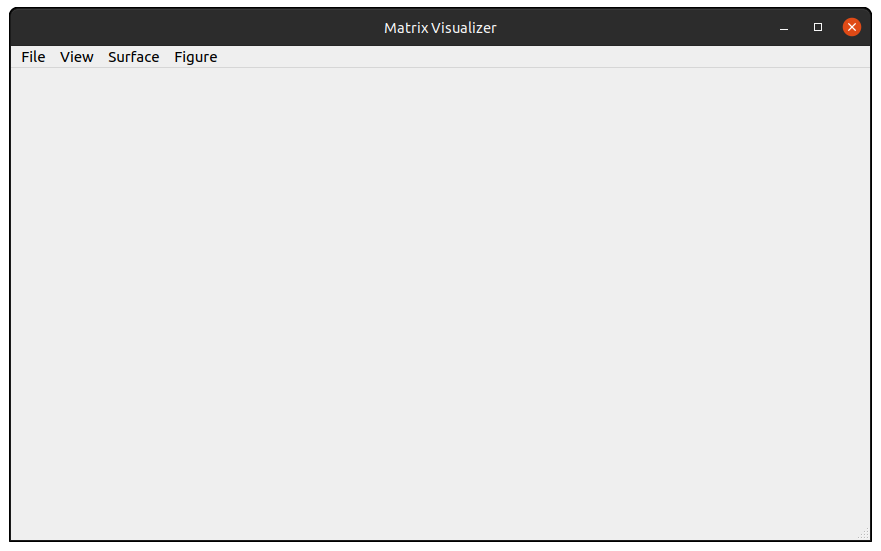
\includegraphics[width=0.8\textwidth]{images/start.png}
	\caption{интерфейс при запуске}
	\label{start_interface}
\end{figure}

\noindent Контекстное меню включает в себя следующие разделы:
\begin{itemize}
    \item \enquote{File} - меню взаимодействия с файлами и управлениея общим состоянием приложения;
    \item \enquote{View} - меню взаимодействия с отображаемыми трехмерными объектами;
    \item \enquote{Surface} - меню взаимодействия с поверхностями;
    \item \enquote{Figure} - меню взаимодействия с фигурами.
\end{itemize}

Пункты (действия) контекстного меню могут обладать комбинацией клавиш клавиатуры, при нажатии которых данное действие будет выполнено без открытия контекстного меню. При наличии такой комбинации ее можно увидеть справа от имени пункта.

\subsection{Фигуры}
Фигура является базовым и основным типом 3D объекта, которое использует приложение. Она представляет из себя набор вершин (с указанием координат в трехмерном пространстве) и набор связей между этими вершинами. Каждая из вершин имеет свой уникальный (в пределах одной фигуры) идентификатор, а каждая связь является набором двух различных идентификаторов вершин.

Для взаимодействия с фигурами (создание, редактирование и т. п.) предусмотрен раздел контекстного меню \enquote{Figure} (рис.~\ref{figure_menu}).
\begin{figure}[htbp!]
	\centering
	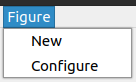
\includegraphics[width=0.2\textwidth]{images/figuremenu.png}
	\caption{меню взаимодействия с фигурами}
	\label{figure_menu}
\end{figure}

\subsubsection{Открытие}
Контекстное меню \enquote{File} (рис.~\ref{file_menu}) располагает пунктом \enquote{Open}, который используется для открытия 3D объектов любого типа. Для открытия фигуры нужно нажать на данный пункт и в окрывшемся диалоге, выбрать фигуру с диска. Обычно фигуры имеют расширение \verb|.xml|.
\begin{figure}[htbp!]
	\centering
	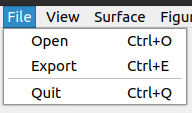
\includegraphics[width=0.2\textwidth]{images/filemenu.png}
	\caption{меню взаимодействия с файлами}
	\label{file_menu}
\end{figure}

После открытия фигура будет отрисована в соответсвующем поле (рис.~\ref{figure}). Имеется возможность открытия нескольких фигур одновременно, при этом обзор будет выбран так, чтобы каждая из открытых фигур целиком поместилась в область отрисовки. 
\begin{figure}[htbp!]
	\centering
	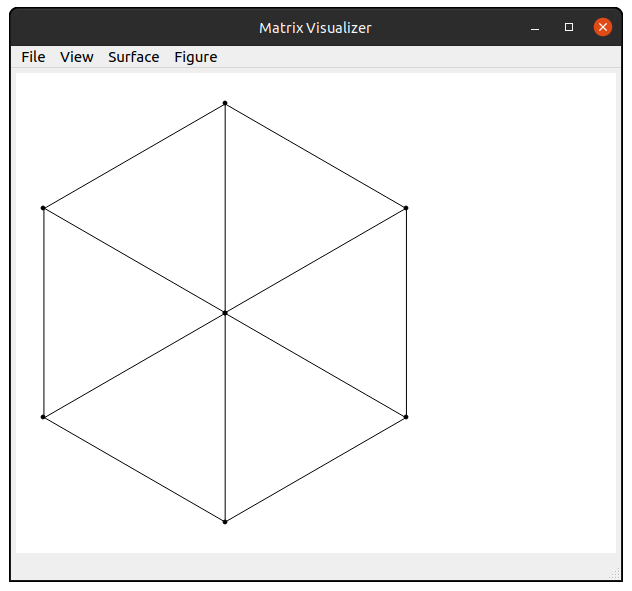
\includegraphics[width=0.7\textwidth]{images/figureopened.png}
	\caption{фигура}
	\label{figure}
\end{figure}

\subsubsection{Создание}
Создание фигуры предполагает добавление вершин и связей между ними. Для того, чтобы создать фигуру необходимо выбрать пункт \enquote{New} в разделе \enquote{Figure}. Будет открыто диалоговое окно для создания / редактирования фигур (рис.~\ref{figure_cfg_new}).

В верхней части интерфейса открывшегося окна можно увидеть поле тэга (\enquote{Tag}) фигуры. Каждая фигура имеет свой уникальный (относительно запущенного сеанса) тэг. Для открытых и новых фигур тэг генерируется автоматически. Его можно изменить, введя в соответсвующее поле новое значение тэга.

Далее располагается флажок \enquote{Hide}. Его включение определит фигуру как скрытую, которая не будет отображена.

Чуть ниже можно заметить поле, в котором могут быть размещены вершины. Для добавления новой вершины необходимо нажать кнопку \enquote{Add}. После добавления хотя бы одной вершины становится доступным их редактирование. Уникальный идентификатор вершин генерируется автоматически. С помощью полей \enquote{Location} можно установить положение вершины в пространстве.
\begin{figure}[htbp!]
	\centering
	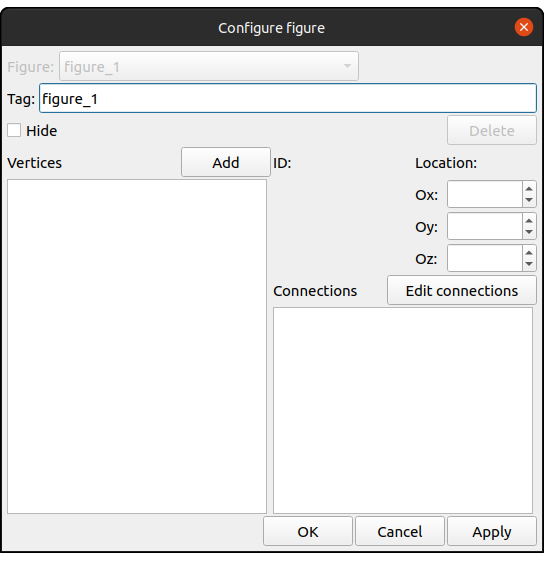
\includegraphics[width=0.6\textwidth]{images/figurecfgnew.png}
	\caption{создание фигуры}
	\label{figure_cfg_new}
\end{figure}

Также у выбранной из списка вершины в поле \enquote{Connections} присутствуют ее связи с другими вершинами. Их можно редактировать, нажав на \enquote{Edit connections}. После нажатия данной кнопки будет открыто новое диалоговое окно - панель добавления межвершинных связей (рис.~\ref{add_connections}).

\begin{figure}[htbp!]
	\centering
	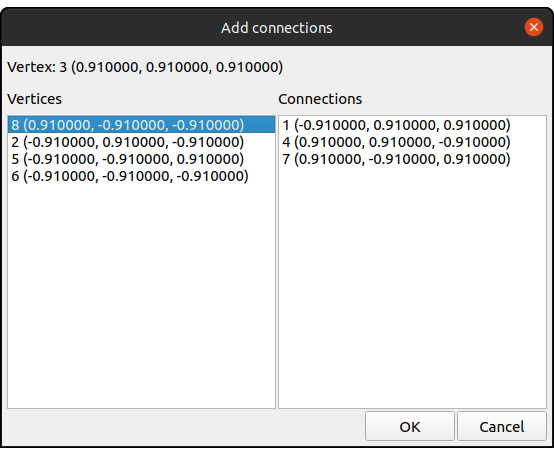
\includegraphics[width=0.6\textwidth]{images/addconnections.png}
	\caption{панель добавления межвершинных связей}
	\label{add_connections}
\end{figure}

Сверху располагается вершина, связи которой редактируются в данном окне. В списке слева (\enquote{Vertices}) присутствуют имеющиеся, но не связанные с данной, вершины. Список справа есть список уже установленных связей. Для удаления вершины из одного списка и добавления в другой, достаточно двойного клика левой кнопкой мыши по соответсвующей вершине. После окончания редактирования можно принять осуществленные изменения с помощью кнопки \enquote{OK} или же отклонить (отменить) с помощью кнопки \enquote{Cancel}.
 
 Для удаления какой-либо вершины необходимо выбрать ее в списке и правой кнопкой мыши нажать на нее. В открывшемся контекстном меню нужно выбрать единственный пункт \enquote{Delete}.
 
\subsubsection{Редактирование}
Редактирование фигур представляет собой процесс идентичный их созданию. Для их редактирования нужно открыть пункт \enquote{Configure} в разделе \enquote{Figure}. В появившемс, ранее рассмотренном, окне создания/редактирования фигур (рис.~\ref{figure_cfg}) в верхней части интерфейса стал доступен выбор фигуры для редактирования. При смене фигуры, все данные (тэг, вершины и т. п.) будут перезагружены.

\begin{figure}[htbp!]
	\centering
	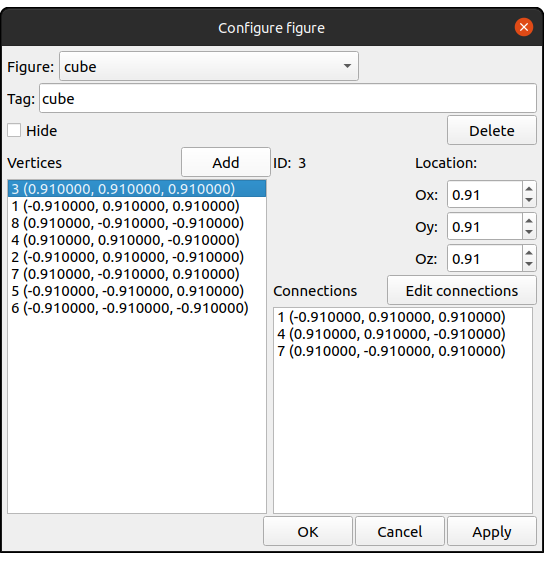
\includegraphics[width=0.6\textwidth]{images/figurecfg.png}
	\caption{панель редактирования фигур}
	\label{figure_cfg}
\end{figure}

Также присутствует кнопка \enquote{Delete}, при нажатии на которую фигура удаляется из текущего сеанса. В случае, если фигура не была сохранена прежде, будет открыто диалоговое окно, предлагающее сделать сохранение (рис.~\ref{not_saved_warning_delete}). В случае подтверждения сохранения будет открыта панель сохранения.

\begin{figure}[htbp!]
	\centering
	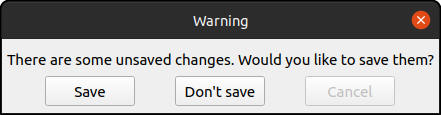
\includegraphics[width=0.6\textwidth]{images/notsavedwarning.png}
	\caption{предупреждение о несохраненных изменениях (при удалении)}
	\label{not_saved_warning_delete}
\end{figure}

Чтобы принять изменения, но не закрывать панель редактирования необходимо нажать \enquote{Apply}. Для принятия и закрытия панели - \enquote{OK}. Для закрытия панели без принятия изменения - \enquote{Cancel}.

\subsubsection{Сохранение}
Сохранение производится при выборе пункта \enquote{Export} в разделе \enquote{File} контекстного меню, а также при попытке удаления из сеанса несохраненной фигуры и завершении сеанса при наличии несохраненных фигур.

Панель сохранения фигур (рис.~\ref{export}) содержит список фигур, которые можно выбрать для сохранения. Далее указывается путь сохранения. Если фигура была открыта, путь сохранения установлен равный открытому пути, следовательно, при сохранении прежний файл будет перезаписан новым. Если же фигура была создана или преобразована из другого типа (напр. поверхность), сохранение будет невозможно без самостоятельного выбора пути. Самостоятельный выбор пути осуществляется по нажатию кнопки \enquote{Browse}. При выбранном пути кнопка \enquote{Export} становится активной и при ее нажатии, произойдет сохранение. Также возможна отмена сохранения по нажатию на \enquote{Cancel}.
\begin{figure}[htbp!]
	\centering
	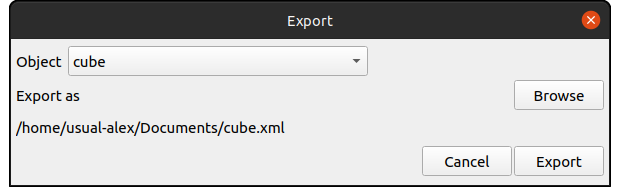
\includegraphics[width=0.7\textwidth]{images/export.png}
	\caption{панель сохранения фигур}
	\label{export}
\end{figure}

\subsection{Поверхности}
Поверхности - поддерживаемый тип 3D объекта, представляющий собой матрицу чисел, которые являются значением функции двух переменных. Аргументы же ее в виде расстояния между точками по двум осям генерируются приложением или задаются вручную. Имеется возможность нормализации значений, которая представляет собой приведение значений функции к заданному диапазону. Формат файла, в котором содержатся поверхности - \verb|.csv|.

При загрузке поверхности, она автоматически конвертируется в фигуру, следовательно, после этого, к ней применимы все действия, применимые к фигурам. Также она приобретает статус несохраненной, так как не была сохранена в формате фигуры.

Раздел контекстного меню для работы с поверхностями - \enquote{Surface} (рис.~\ref{surface_menu}).
\begin{figure}[htbp!]
	\centering
	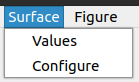
\includegraphics[width=0.3\textwidth]{images/surfacemenu.png}
	\caption{меню взаимодействия с поверхностями}
	\label{surface_menu}
\end{figure}

\subsubsection{Открытие}
Открытие поверхности происходит аналогично открытию фигуры. При помощи пункта \enquote{Open} контекстного меню \enquote{File} происходит выбор файла для открытия. Однако так как набор значений в файле представляет из себя лишь набор высот каждой из точек, для выбора расстояния между ними после выбора файла будет открыта панель редактирования поверхности с частичным доступом (рис.~\ref{surface_cfg_open}).
\begin{figure}[htbp!]
	\centering
	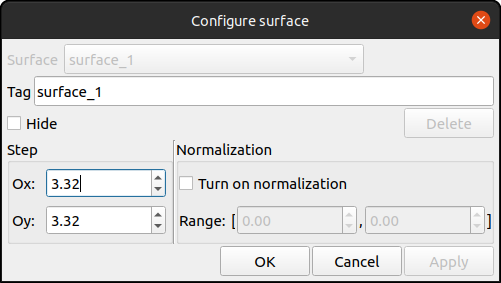
\includegraphics[width=0.6\textwidth]{images/surfacecfgopening.png}
	\caption{панель редактирования поверхности (при открытии)}
	\label{surface_cfg_open}
\end{figure}

Расстояние между точками регулируется двумя полями в разделе \enquote{Step}. В соседнем разделе \enquote{Normalization} можно включить нормализацию путем отметки флажка \enquote{Turn on normalization}. После чего станет доступен выбор диапазона нормализации.

В данной панели доступен также выбор тега в верхней части интерфейса, при этом тэг поверхности дублируется в тэг сконвертированной из этой поверхности фигуры, следовательно, он должен быть уникален среди фигур в данном сеансе.

Ниже поля задания тэга расположен флажок \enquote{Hide} аналогичный данному флажку в фигуре.

После настройки параметров поверхности необходимо принять изменения кнопкой \enquote{OK}. Данное действие закроет панель редактирования и произведет отрисовку поверхности (рис.~\ref{surface}). Нажатие же кнопки \enquote{Cancel}, вернет приложение в состояние, в котором оно прибывало до открытия фигуры.

\begin{figure}[htbp!]
	\centering
	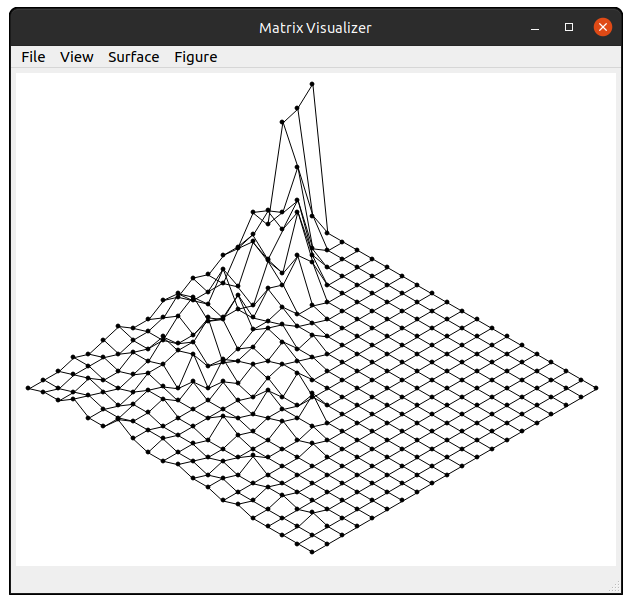
\includegraphics[width=0.7\textwidth]{images/surfaceopened.png}
	\caption{поверхность}
	\label{surface}
\end{figure}

\subsubsection{Просмотр}
В приложении доступен просмотр значений функции двух переменных открытой поверхности. Для этого нужно выбрать пункт \enquote{Values} контекстного меню \enquote{Surface}. Данный пункт отобразит панель просмотра значений поверхности (рис.~\ref{surface_view}).

\begin{figure}[htbp!]
	\centering
	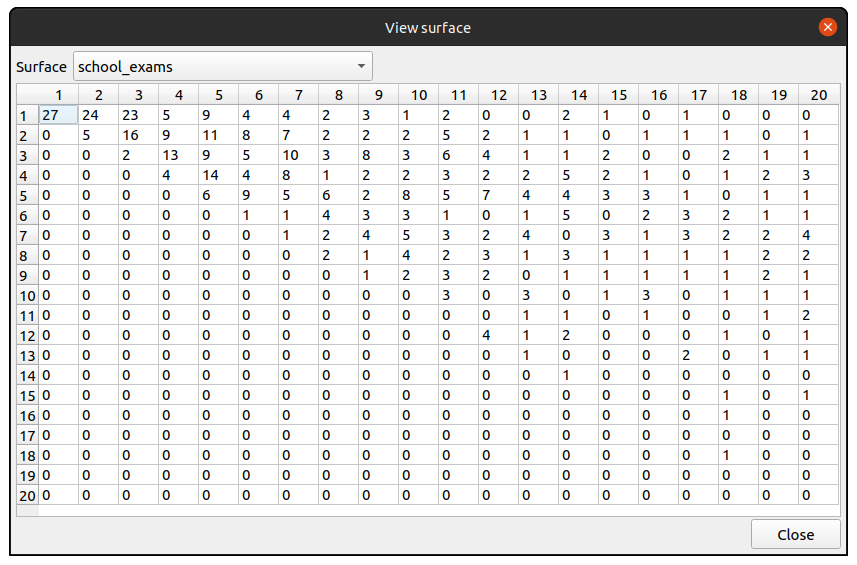
\includegraphics[width=0.7\textwidth]{images/surfaceview.png}
	\caption{панель просмотра значений поверхности}
	\label{surface_view}
\end{figure}

В данной панели в верхней части интерфейса доступен выбор поверхности, значения которой необходимо просмотреть. Значения отображаются в виде таблице в том порядке, в котором они присутствуют в поверхности.

\subsubsection{Редактирование}
Редактирования поверхности, так же, как и редактирование фигуры идентично ее первоначальной настройке. Открыть панель редактирования (рис.~\ref{surface_cfg}) поверхности можно с помощью пункта \enquote{Configure} контекстного меню \enquote{Surface}.

\begin{figure}[htbp!]
	\centering
	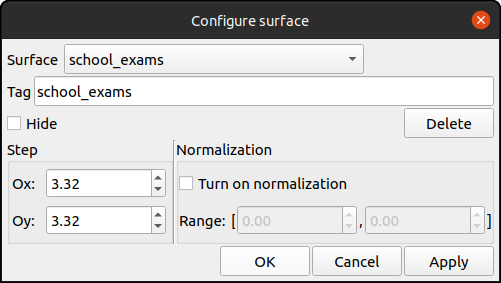
\includegraphics[width=0.6\textwidth]{images/surfacecfg.png}
	\caption{панель редактирования поверхности}
	\label{surface_cfg}
\end{figure}

В данной панели доступен выбор поверхности для редактирования, а также кнопка удаления \enquote{Delete}, которая удалит как поверхность, так и соответствующую ей фигуру.

Так же, как и в панели редактирования фигур, в нижней части интерфейса присутствуют три кнопки:
\begin{itemize}
    \item \enquote{OK} - применить изменения и закрыть панель;
    \item \enquote{Cancel} - не применять изменения и закрыть панель;
    \item \enquote{Apply} - применить изменения, но не закрывать панель.
\end{itemize}

\subsection{Операции}
В приложении доступен функционал для оперирования видимыми фигурами. Данный функционал заключен в контекстное меню \enquote{View} (рис.~\ref{view_menu}).

\begin{figure}[htbp!]
	\centering
	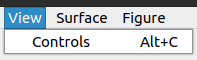
\includegraphics[width=0.3\textwidth]{images/viewmenu.png}
	\caption{меню взаимодействия с видимыми фигурами/поверхностями}
	\label{view_menu}
\end{figure}

\subsubsection{Панель управления}
Для управления положением фигуры в пространстве используется панель управления (рис.~\ref{controls}). Доступ к ней происходит через пункт \enquote{Controls} раздела \enquote{View} контекстного меню. Она представляет из себя набор элементов управления фигурой, выбранной в верхней части интерфейса.

\begin{figure}[htbp!]
	\centering
	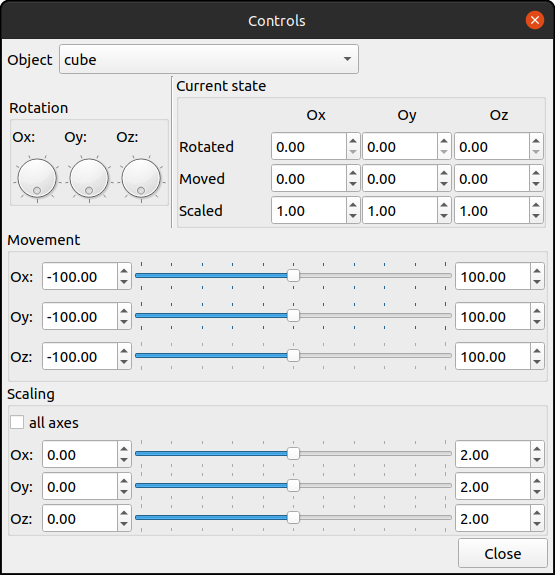
\includegraphics[width=0.6\textwidth]{images/controls.png}
	\caption{панель управления}
	\label{controls}
\end{figure}

Во время работы с панелью управления происходит изменение положения фигуры в пространстве и соответствующее изменение ее координат, которое придает фигуре статус наличия несохраненных изменений. При этом ее положение будет сохранено на протяжении всего ее существования в данном сеансе.

Численные значения положения фигуры в пространстве представлены в таблице \enquote{Current state}. При этом они могут быть изменены прямым внесением изменений в данную таблицу.

\subsubsection{Масштабирование}

Масштабирование фигуры выполняется набором управляющих элементов в нижней части панели управления. Они представляют из себя ползунок, начальные и конечные положения которого определяются соответствующими полями. Поля масштабирования в разделе \enquote{Current state} также ограничены пограничными полями ползунков. По умолчанию каждая фигура имеет масштаб равный \verb|1| по всем осям. Масштабирование не может иметь значение меньше или равное нулю. Результат масштабирования представлен на рис.~\ref{scaling}.

\begin{figure}[htbp!]
	\centering
	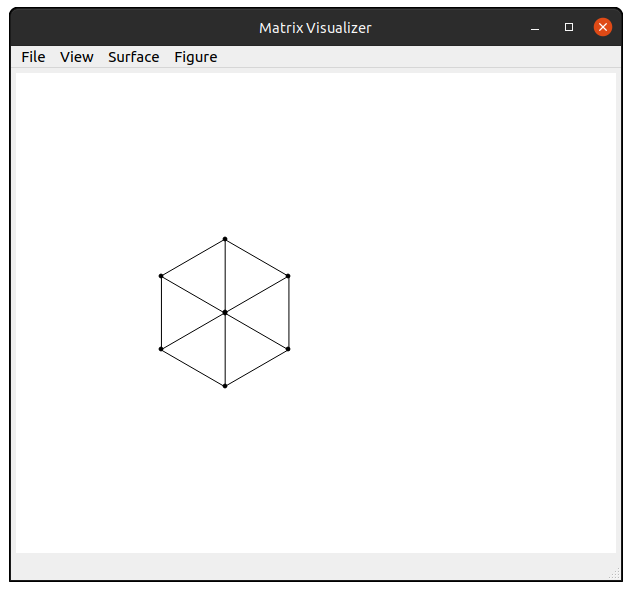
\includegraphics[width=0.6\textwidth]{images/scaling.png}
	\caption{масштабирование}
	\label{scaling}
\end{figure}

Присутствует возможность масштабирования по всем осям одновременно. Для этого необходимо установить флажок \enquote{all axes}. После его установления, масштабирование будет регулироваться единственным ползунком и единственным полем в разделе \enquote{Current state} (рис.~\ref{contols_all}).

\begin{figure}[htbp!]
	\centering
	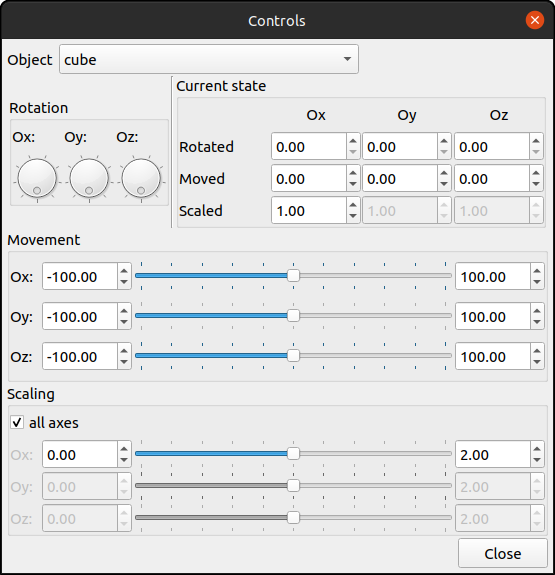
\includegraphics[width=0.6\textwidth]{images/controlsallaxes.png}
	\caption{масштабирование по всем осям (включено)}
	\label{contols_all}
\end{figure}

\subsubsection{Вращение}
Вращение фигуры регулируется тремя дисками в разделе \enquote{Rotation}, а также соответсвующими поялми в \enquote{Current state}. Вращение происходит в пределах от \verb|0| до \verb|360| и измеряется в градусах. Пример вращения показан на рис.~\ref{rotation}.

\begin{figure}[htbp!]
	\centering
	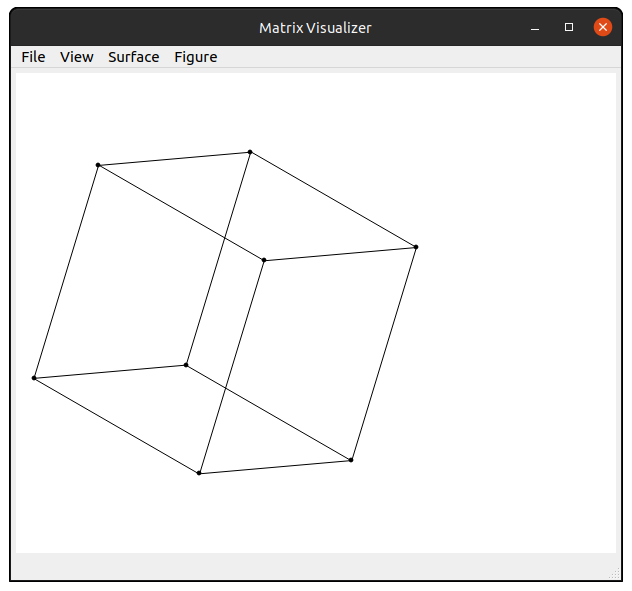
\includegraphics[width=0.6\textwidth]{images/rotation.png}
	\caption{вращение}
	\label{rotation}
\end{figure}

\subsubsection{Перемещение}
Перемещение управляется аналогично масштабированию за исключением того, что может иметь пределы на всей числовой оси. Пример перемещения продемонстрирован на рис.~\ref{movement}.
\begin{figure}[htbp!]
	\centering
	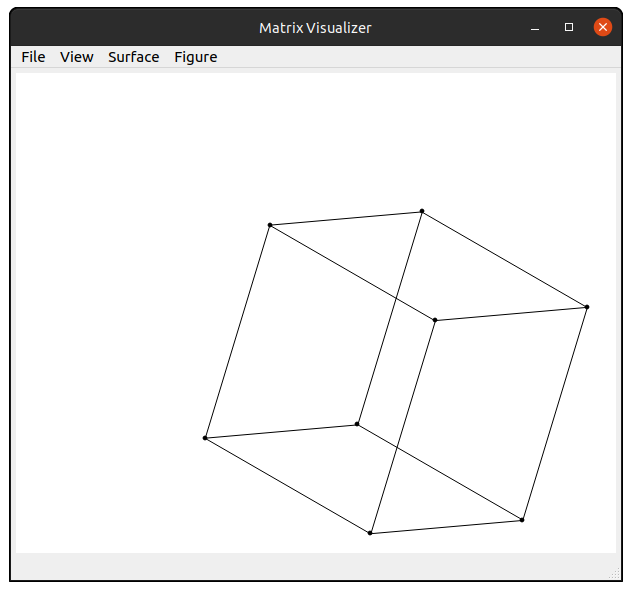
\includegraphics[width=0.6\textwidth]{images/movement.png}
	\caption{Перемещение}
	\label{movement}
\end{figure}

\subsection{Завершение работы}
Закрытие приложения возможно либо классическим путем через кнопку \verb|x|, расположение которой определяется операционной системой, либо через выбор пункта \enquote{Quit} раздела \enquote{File} контекстного меню. В обоих случаях при наличии несохраненных изменений будет открыто диалоговое окно (рис.~\ref{not_saved_warning}), предупреждающее об этом и предоставляющее возможность их сохранить и лишь после этого закрыть приложение.
Он предполагает выбор один из трех вариантов:
\begin{itemize}
    \item \enquote{Save} - сохранить и закрыть приложение;
    \item \enquote{Don't save} - не сохранять и закрыть приложение;
    \item \enquote{Cancel} - не сохранять и отменить закрытие приложения.
\end{itemize}

\begin{figure}[htbp!]
	\centering
	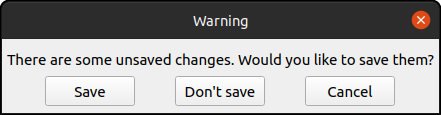
\includegraphics[width=0.6\textwidth]{images/fullnotsavedwarning.png}
	\caption{предупреждение о несохраненных изменениях}
	\label{not_saved_warning}
\end{figure}

\section{Исходный код}
Исходный код к данной лабораторной работе можно найти по \href{https://git.iu7.bmstu.ru/sgn3-prog/sgn3-prog-labs-2019/sgn3-prog-labs-2019-kostarevalexander/-/tree/master/lw-7}{данной ссылке}.


\end{document}
